\documentclass{beamer}
\setbeamertemplate{caption}[numbered]

\setbeamertemplate{headline}{}
\setbeamertemplate{blocks}{shadow=false}
\setbeamertemplate{footline}{}

\usepackage[citations,footnotes,definitionLists,hashEnumerators,smartEllipses,tightLists=false,hybrid]{markdown}
\usepackage{textpos}
\usepackage{lmodern} % http://ctan.org/pkg/lm
\usepackage{booktabs,multirow}
\usepackage{tcolorbox}

\usepackage{scalerel,stackengine}
\stackMath
\newcommand\reallywidehat[1]{%
\savestack{\tmpbox}{\stretchto{%
  \scaleto{%
    \scalerel*[\widthof{\ensuremath{#1}}]{\kern-.6pt\bigwedge\kern-.6pt}%
    {\rule[-\textheight/2]{1ex}{\textheight}}%WIDTH-LIMITED BIG WEDGE
  }{\textheight}% 
}{0.5ex}}%
\stackon[1pt]{#1}{\tmpbox}%
}
\parskip 1ex

\usetheme{Marburg} %%%% theme
\usefonttheme{structurebold} %%%% choose from: serif, professionalfonts, structurebold, structureitalicserif, structuresmallcapsserif
\usecolortheme{lily}  %%% choose theme color from: albatross, beaver, beetle, crane, default, dolphin, dove, fly, lily, orchid, rose, seagull, seahorse, sidebartab, structure, whale, wolverine

%% \beamertemplatenavigationsymbolsempty                                           
\definecolor{mycolTop}{RGB}{4, 40, 120}
\definecolor{mycolBottom}{RGB}{26, 148, 196}
%\makeatletter
\setbeamertemplate{sidebar canvas right}[vertical shading][top=mycolTop, bottom=mycolBottom]
%\makeatother
\setbeamerfont{section in sidebar}{size=\fontsize{6}{6}\selectfont} %%% set font size and row space
\setbeamerfont{subsection in sidebar}{size=\fontsize{6}{6}\selectfont}
%%\setbeamerfont{section in sidebar shaded}{size=\fontsize{2}{2}\selectfont}


\usepackage{graphicx} % Allows including images
\usepackage{booktabs} % Allows the use of \toprule, \midrule and \bottomrule in tables
\usepackage{subcaption}
\usepackage{amsmath,amsfonts,amsthm,bm} 
\usepackage[square,sort,comma]{natbib}

%\usepackage{natbib} 
%\bibliographystyle{apalike}

\usepackage{listings,lstautogobble}
\usepackage{xcolor}
\definecolor{RoyalBlue}{cmyk}{1, 0.50, 0, 0}
\lstset{language=R,
	keywordstyle=\color{RoyalBlue},
	basicstyle=\normalsize\ttfamily,
	commentstyle=\ttfamily\itshape\color{gray},
	stringstyle=\ttfamily,
	showstringspaces=false,
	breaklines=true,
	frameround=ffff,
	frame=single,
	rulecolor=\color{black},
	autogobble=true
}


\newcommand{\iid}{\textrm{i.i.d.\ }}
\newcommand{\E}{\mathrm{E}}
\newcommand{\Var}{\mathrm{Var}}
\newcommand{\Cov}{\mathrm{Cov}}
\newcommand{\Corr}{\mathrm{Corr}}
\newcommand{\tr}{\mathrm{tr}}
\newcommand\inv[1]{#1\raisebox{1.15ex}{$\scriptscriptstyle-\!1$}}


%----------------------------------------------------------------------------------------
%	TITLE PAGE
%----------------------------------------------------------------------------------------

\title[]{Data Visualisation Using \texttt{R}} 

\subtitle{\textcolor{magenta}{Lecture-3}}

\author[]{Suman Rakshit} % Your name
\institute[School of EECMS, Curtin University] % Your institution as it will appear on the bottom of every slide, may be shorthand to save space
{
	\textcolor{magenta}{School of EECMS, Curtin University} % Your institution for the title page
	%\medskip
	%\textit{abc@abc.com} % Your email address
}
%\date{14 September, 2020, SAGI Symposium} % Date, can be changed to a custom date

\titlegraphic{
\includegraphics[width=0.4\textwidth,
height=0.18\textheight]{PlotsLec3/CURTIN}}

\begin{document}



\begin{frame}
	\titlepage % Print the title page as the first slide
\end{frame}


\addtobeamertemplate{frametitle}{}{%
	\begin{textblock*}{100mm}(0\textwidth,8cm)
		
\includegraphics[height=0.8cm,width=2cm]{PlotsLec3/CURTIN}
\end{textblock*}}




%----------------------------------------------------------------------------------------
%	PRESENTATION SLIDES
%----------------------------------------------------------------------------------------

%------------------------------------------------ 
\section{Outline}
\begin{frame}[t]\frametitle{Outline}
\begin{enumerate}
\item A quick review
\item Deep dive into themes layer
\item Key theme element-1: Text elements
\item Key theme element-2: Line elements
\item Key theme element-3: Rectangles
\item Creating custom themes
\item Ggplot-2 and Ggthemes in-built themes
\item Important scale functions
\item Summary
\end{enumerate}
\end{frame}

\section{Quick review}
\setbeamercovered{transparent}
\begin{frame}\frametitle{A quick recap of Ggplot2 basics}
\begin{itemize}
\item Three most important components for any visualisation are: (i) \textcolor{blue}{data} (ii) \textcolor{blue}{aesthetic mapping} and (iii) \textcolor{blue}{geometry}.
\vspace{0.3in}
\item<2-> \textcolor{blue}{Aesthetic mapping} is performed using the function \texttt{\textcolor{red}{aes(x, y, color, fill, shape, size, alpha)}}.
\vspace{0.3in}
\item<3-> \textcolor{blue}{Geometry} corresponds to \textit{chart type}, and is specified using \texttt{\textcolor{red}{geom$\_\star$}\textcolor{red}{()}}, where a chart type is specified in place of \textcolor{red}{$\star$}.
\vspace{0.3in}
\item<4-> \textcolor{blue}{Visible attributes} are specified outside \texttt{\textcolor{red}{aes()}} and, most often, inside the \texttt{\textcolor{red}{geom$\_\star$}\textcolor{red}{()}} function. 
\end{itemize}
\end{frame}

\section{Deep dive into themes}
%\setbeamercovered{transparent}
\begin{frame}{Deep dive into \textbf{\textcolor{red}{themes}} layer}
\Large
\begin{itemize}
\item The \textcolor{blue}{themes} layer provides all \textcolor{blue}{non-data} related visible attributes -- \texttt{\textcolor{red}{theme()}} allows you to \textcolor{blue}{modify all non-data ink} in your visualisation.

\vspace{0.3in}

\item Three main visual elements of \textcolor{blue}{themes} layer: 
\begin{enumerate}
\Large
\item \texttt{\textcolor{red}{text}}: modify using \texttt{\textcolor{red}{element}$\_$\textcolor{red}{text()}}
\item \texttt{\textcolor{red}{line}}: modify using \texttt{\textcolor{red}{element}$\_$\textcolor{red}{line()}}
\item \texttt{\textcolor{red}{rectangle}}: modify \texttt{\textcolor{red}{element}$\_$\textcolor{red}{rect()}}
\end{enumerate}
\end{itemize}
\end{frame}

\begin{frame}\frametitle{\textbf{\textcolor{red}{Important}}: \texttt{\textcolor{red}{element$\_\star$()}} functions!}
\begin{figure}
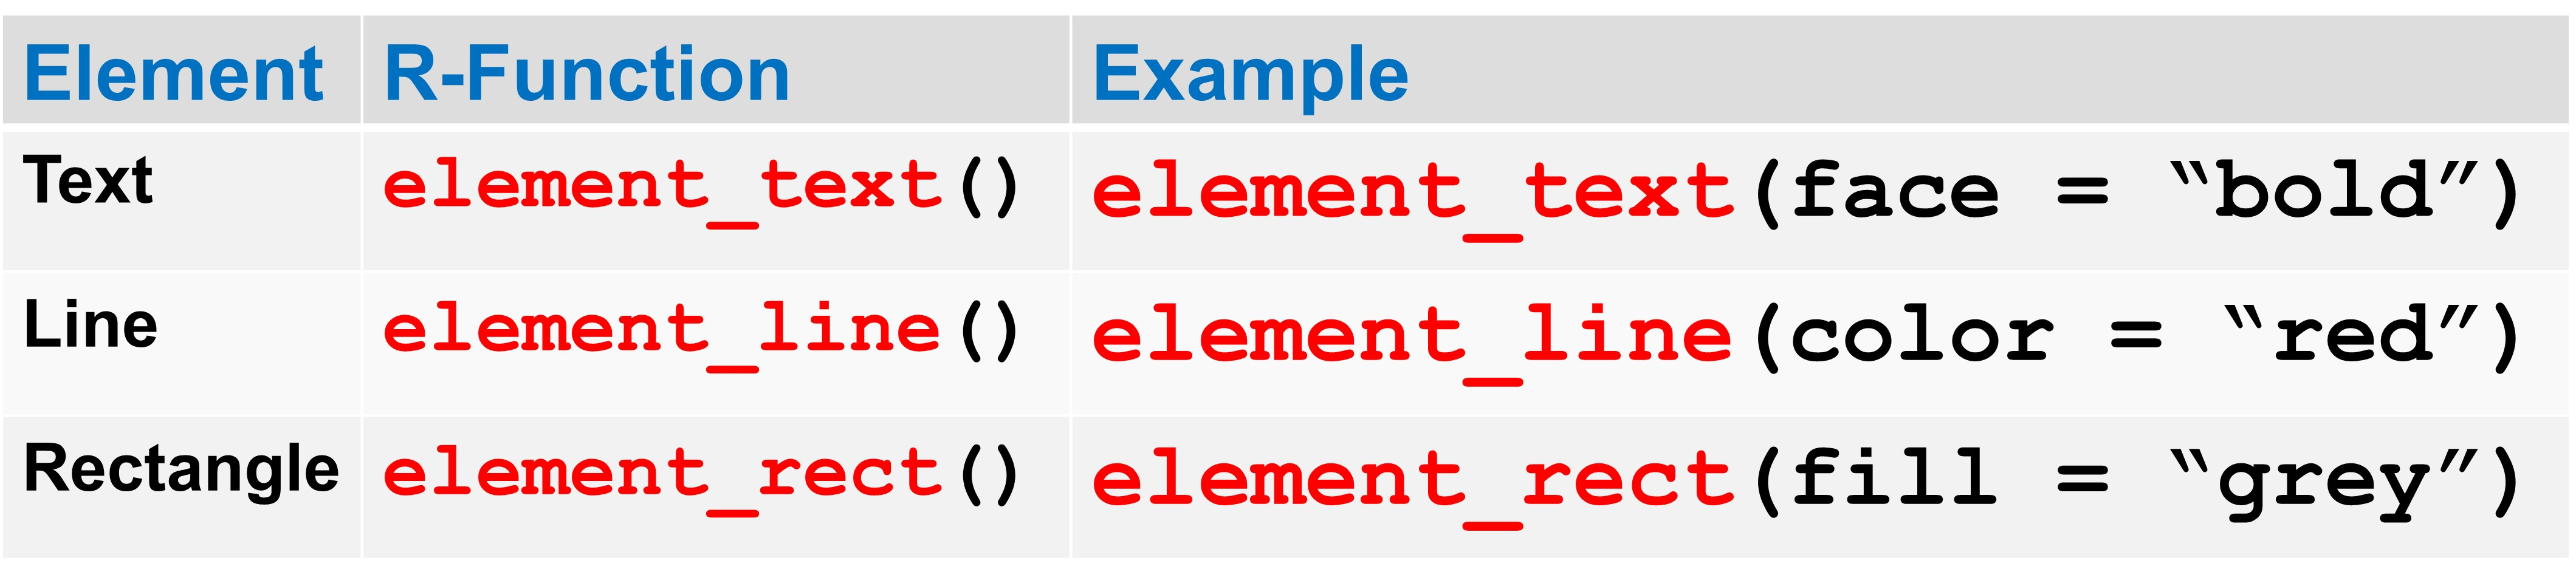
\includegraphics[width=0.99\linewidth]{PlotsLec3/ElementFunctions2}
\end{figure}
One important \texttt{\textcolor{red}{element$\_\star$()}} function is \texttt{\textcolor{red}{element$\_$blank()}} --- this function removes any themes-based visual element.

Example: \texttt{\textcolor{red}{theme(\textcolor{blue}{panel.grid} = element$\_$blank())}} \\
removes all panel grid-lines.
\end{frame}

\section{Text elements}
\begin{frame}{\texttt{\textcolor{red}{text}} element hierarchy structure}
\begin{figure}
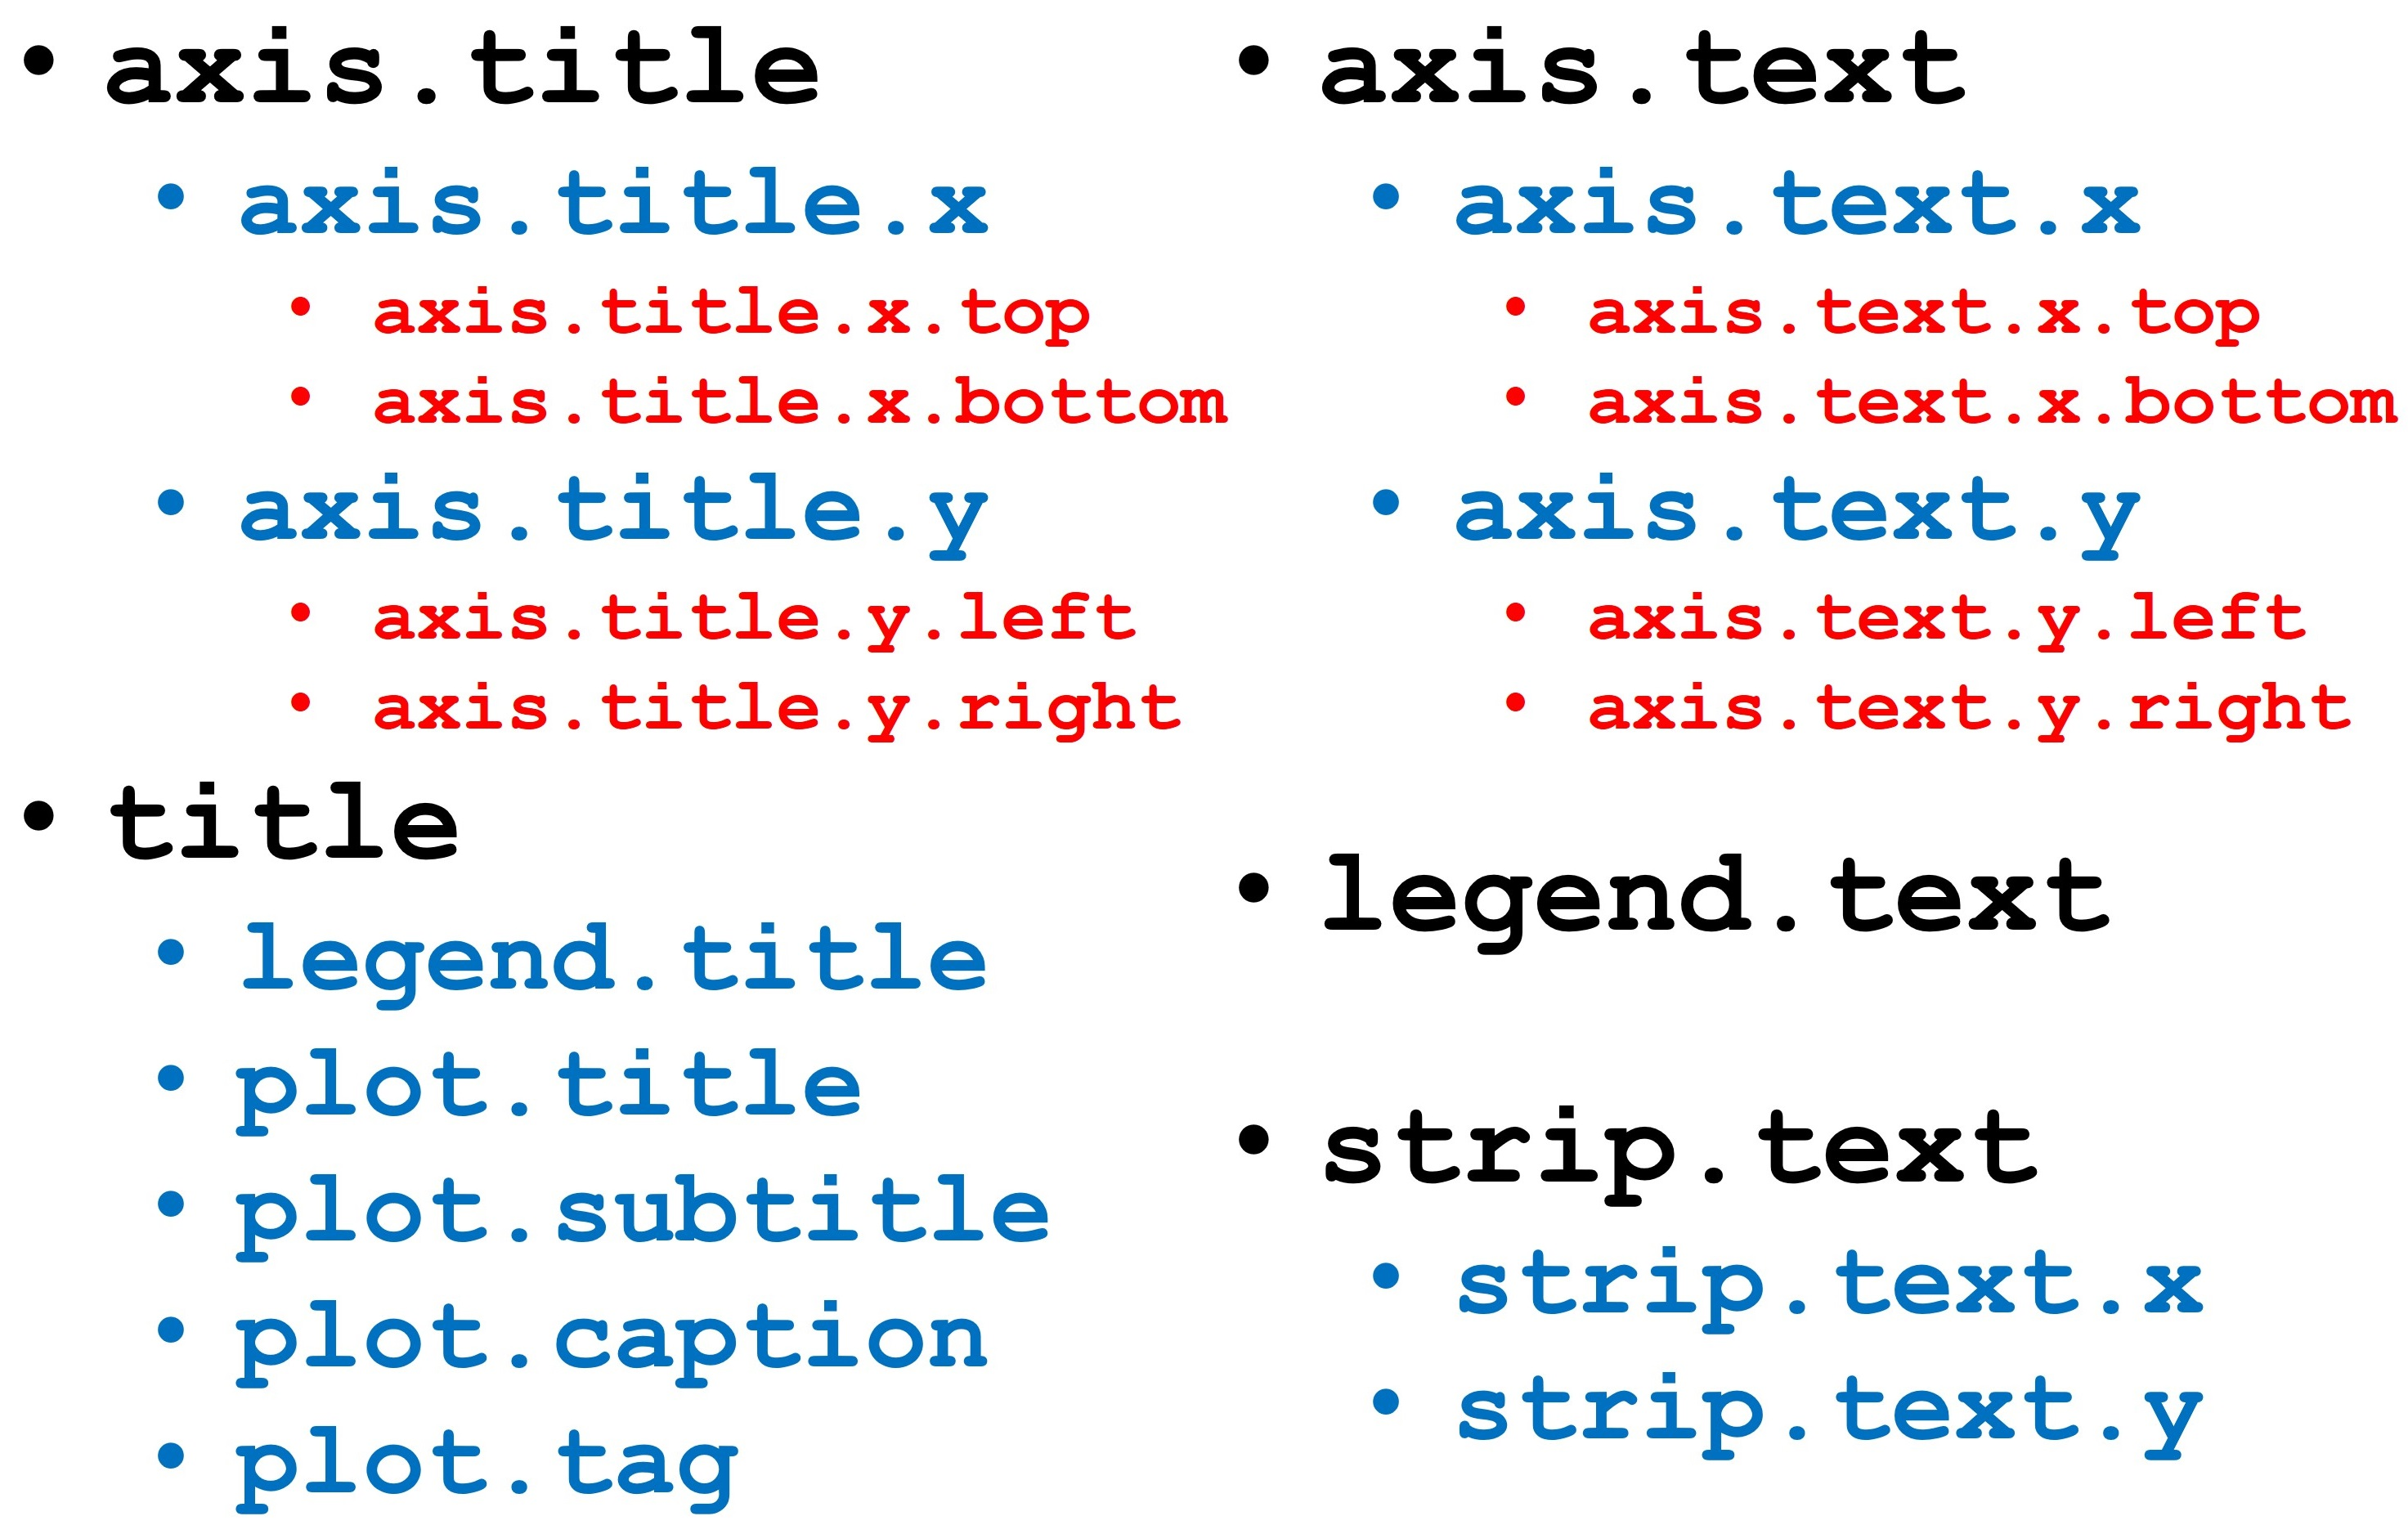
\includegraphics[width=0.99\linewidth]{PlotsLec3/TextThemeElements2}
\end{figure}
\end{frame}

\begin{frame}{Visualize \texttt{\textcolor{red}{text}} elements in a plot}
\begin{figure}
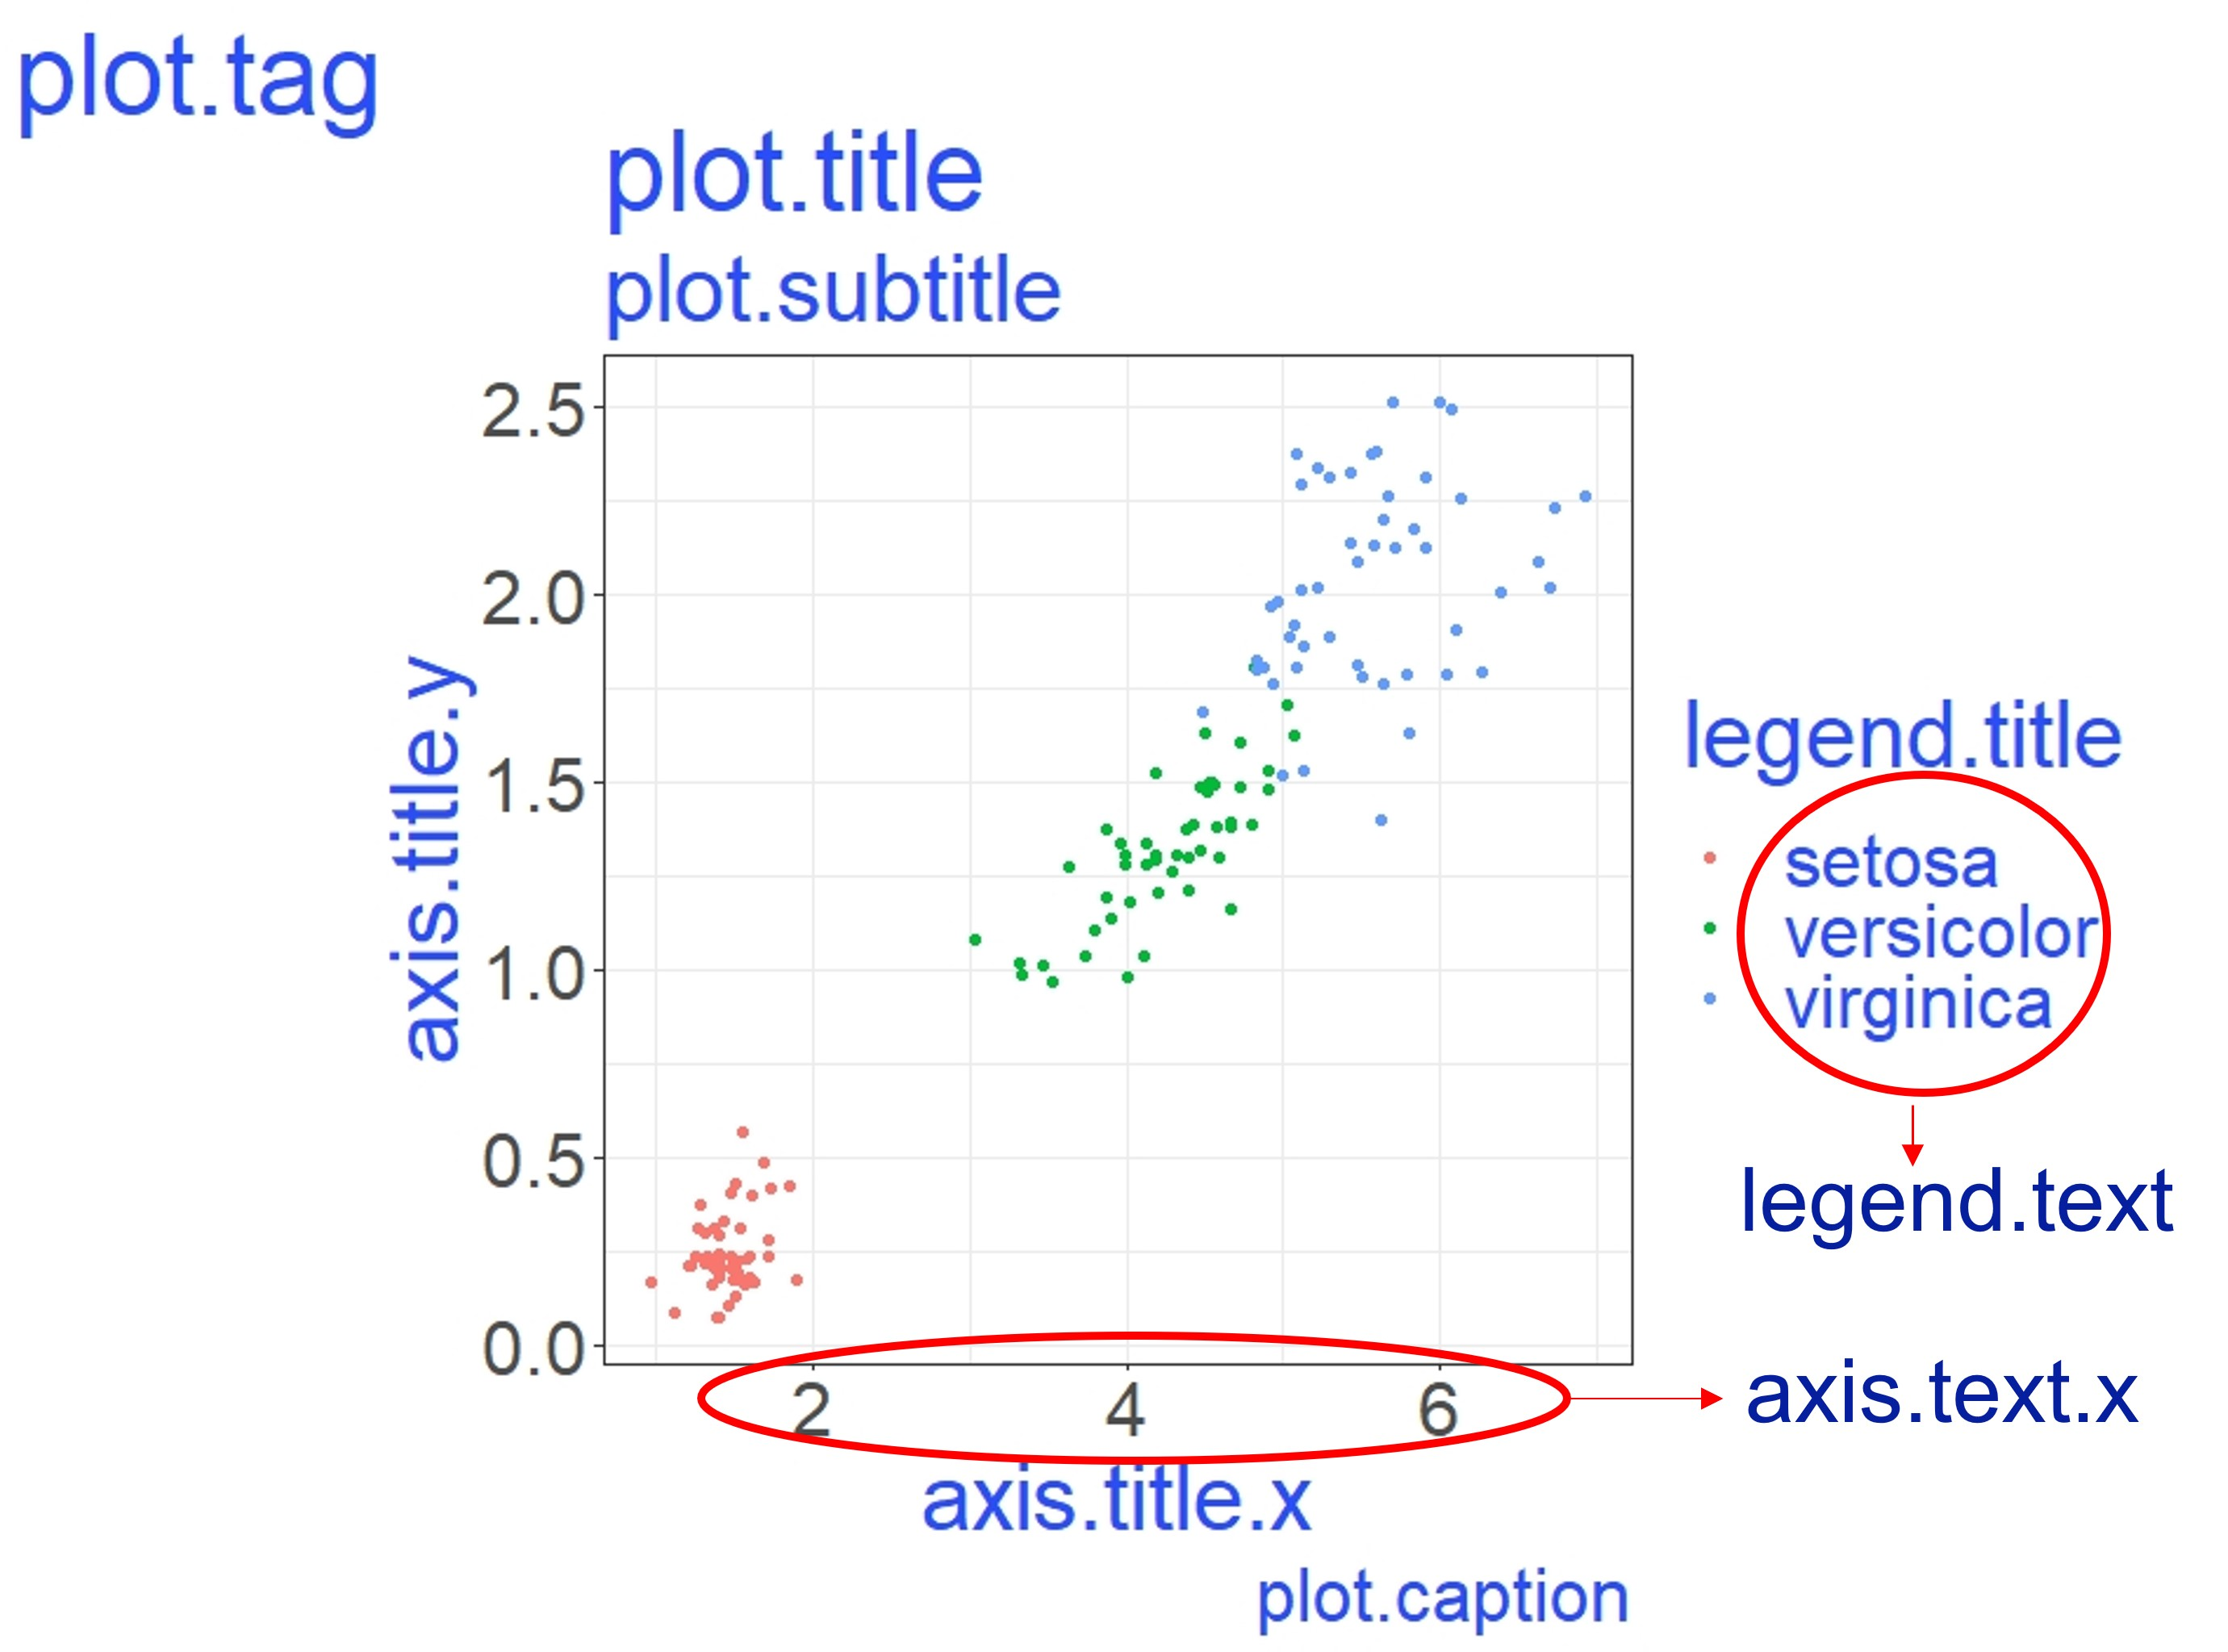
\includegraphics[width=0.99\linewidth]{PlotsLec3/TextThemeElements3}
\end{figure}
\end{frame}

\begin{frame}[fragile]{RCode to specify \texttt{\textcolor{red}{text}} elements}
%\lstset{basicstyle=\tiny\ttfamily}
\begin{lstlisting}
# Standard scatter plot
ggplot(iris, aes(Petal.Length, Petal.Width, color=Species)) +
geom_point() + theme_bw() +
# Specify text elements using labs()
labs(color = "legend.title",
     title = "plot.title",
     subtitle = "plot.subtitle",
     caption = "plot.caption",
     tag = "plot.tag",
     x = "axis.title.x",
     y = "axis.title.y") +
# Modify text size and color
theme(text = element_text(size = 30, 
                     color = "#2A4DFA"))
\end{lstlisting}
\end{frame}

\begin{frame}{Visualize \textcolor{red}{\texttt{strip.text}}}
\begin{figure}
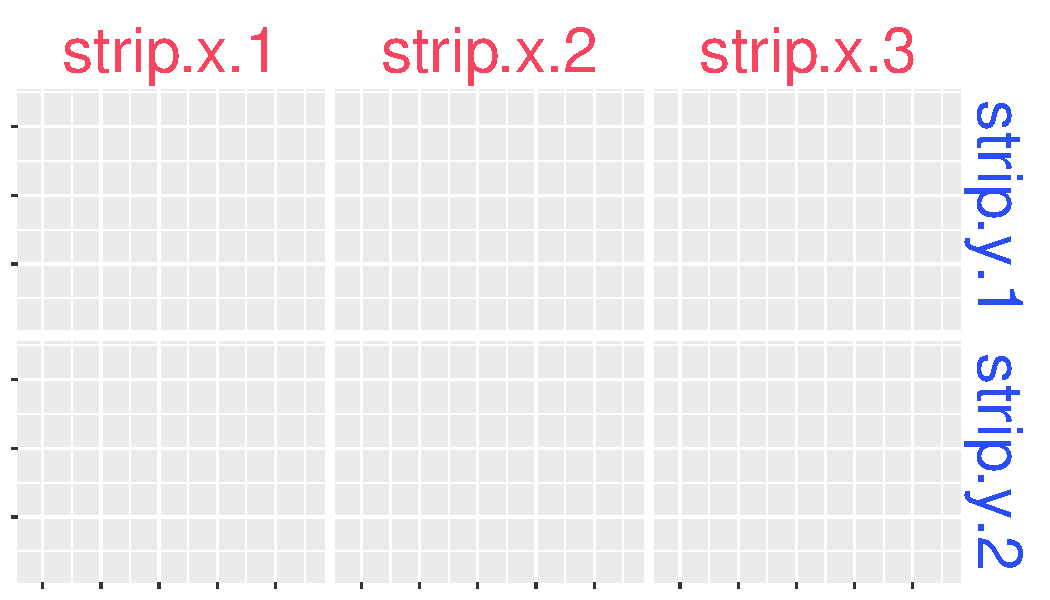
\includegraphics[width=0.99\linewidth]{PlotsLec3/StripText}
\caption{{\small \textcolor{red}{\texttt{strip.text.x}} and \textcolor{blue}{\texttt{strip.text.y}}}.}
\end{figure}
\end{frame}

\begin{frame}{Modified \textcolor{red}{\texttt{strip.text}}}
We modified the \textcolor{blue}{font family}, \textcolor{blue}{color} and \textcolor{blue}{size} of the \textcolor{red}{\texttt{strip.text}} element in the plot.
\begin{figure}
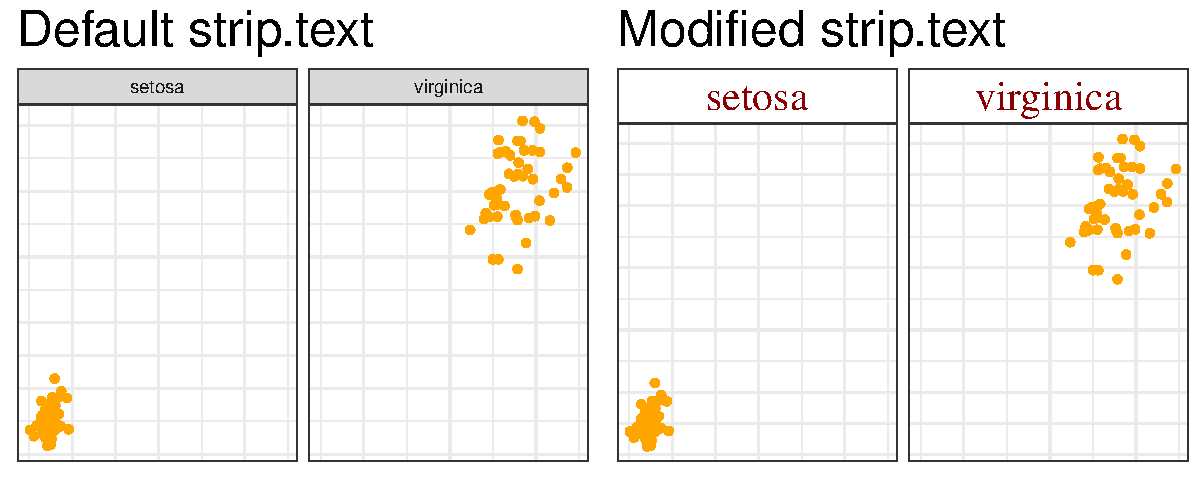
\includegraphics[width=0.99\linewidth]{PlotsLec3/StripText2}
\caption{{\small \textit{Left}: Default \textcolor{red}{\texttt{strip.text}}; \textit{Right}: Font family, color and size are modified of \textcolor{red}{\texttt{strip.text}}}.}
\end{figure}
\end{frame}

\begin{frame}[fragile]{RCode to modify \texttt{\textcolor{red}{strip.text}}}
%\lstset{basicstyle=\Large\ttfamily}
\begin{lstlisting}
# Modify font family, size, and color
theme(strip.text = element_text(
                    family = "serif",
                      size = 20,
                     color = "#8b0000"))
\end{lstlisting}
\end{frame}

\begin{frame}{Modified \textcolor{red}{\texttt{legend.title}} and \textcolor{red}{\texttt{legend.text}}}
%\small
We modified the \textcolor{blue}{font family}, \textcolor{blue}{color} and \textcolor{blue}{size} of \textcolor{red}{\texttt{legend.title}} and  \textcolor{red}{\texttt{legend.text}}.
\begin{figure}
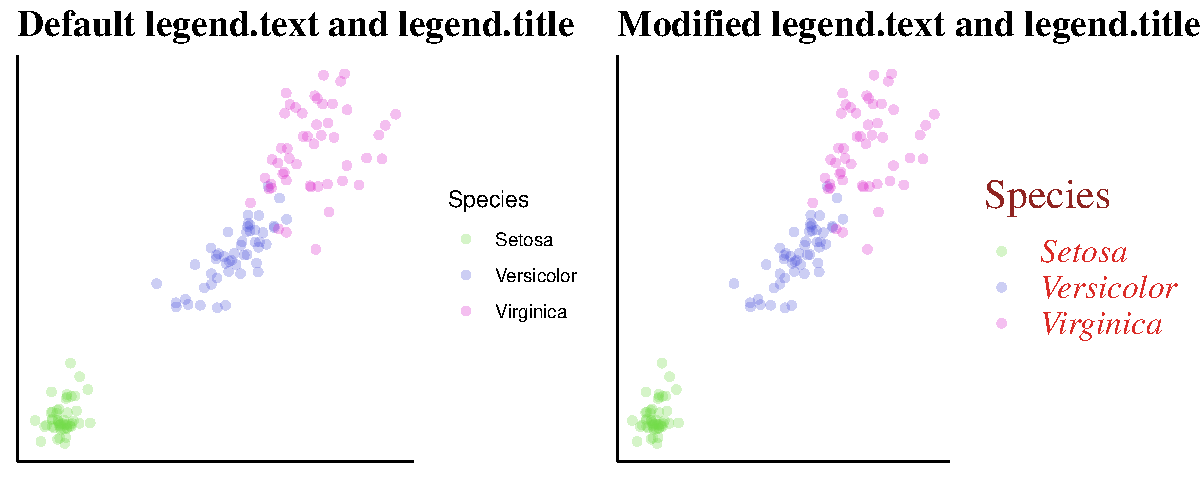
\includegraphics[width=0.99\linewidth]{PlotsLec3/LegText}
\end{figure}
\textcolor{blue}{Can you spot the problem} that still remains with the \textcolor{red}{\texttt{legend guide}}?
\end{frame}

\begin{frame}[fragile]{RCode: modify \texttt{\textcolor{red}{legend}} text elements}
%\lstset{basicstyle=\Large\ttfamily}
\begin{lstlisting}
# Modify font family, size, and color
theme( # modify legend.title
legend.title = element_text(
family = "serif", size = 20, 
     color = "#8F2421"),
     
       # modify legend.text
 legend.text = element_text(
 family = "serif", face = "italic",
 size = 16, color = "#DB2C27"))
\end{lstlisting}
\end{frame}

\setbeamercovered{transparent}
\begin{frame}\frametitle{Fix legend guide using \texttt{\textcolor{red}{guides}} layer}
\Large
\begin{itemize}
\item Sometimes we want the ``\textcolor{blue}{\textit{geoms in the legend}}" to display differently to the ``\textcolor{blue}{\textit{geoms in the plot}}".

\vspace{0.3in}

\item<2-> This is particularly important when the \textcolor{blue}{size} of the points \textcolor{blue}{is small} or the \textcolor{blue}{transparency} of the points \textcolor{blue}{is high}.

\vspace{0.3in}

\item<3-> To modify legend guides, we can use the \texttt{\textcolor{red}{override.aes}} parameter of \texttt{\textcolor{red}{guide}$\_$\textcolor{red}{legend()}}.
\end{itemize}
\end{frame}

\begin{frame}\frametitle{Example: modify legend guides for clarity}
We have \textcolor{red}{increased the size and the value of the alpha attribute} of the points used in the legend guide. 
\begin{figure}
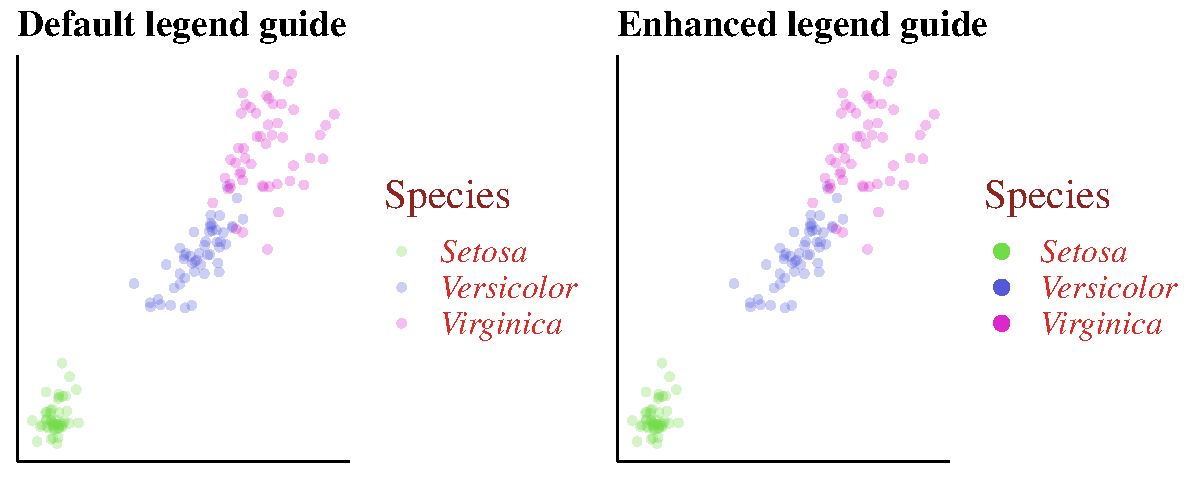
\includegraphics[width=0.99\linewidth]{PlotsLec3/LegGuide}
\caption{\small{\textit{Left}: default legend guide; \textit{Right}: Legend point size has been increased to 3 and alpha value to 1.}}
\end{figure}
\end{frame}


\begin{frame}[fragile]{RCode to modify \texttt{\textcolor{red}{legend guide}}}
%\lstset{basicstyle=\Large\ttfamily}
\begin{lstlisting}
# Create new color guide object
col_guide <- guide_legend(
       override.aes = list(alpha = 1,
                           size = 3))
                                   
# Modify size and alpha of legend points                           
ggplot(iris, aes(Petal.Length, 
                 Petal.Width,
                 color = Species)) +
# Call geom_point() with alpha 0.30
geom_point(alpha = 0.30) +
# Modify the points in the legend guide
guides(color = col_guide)
\end{lstlisting}
\end{frame}

\setbeamercovered{transparent}
\begin{frame}\frametitle{Specify legend position}
\begin{itemize}
\item One of the key tricks to enhance the visualisation is to be creative with the legend position.

\vspace{0.2in}

\item<2-> The easiest way to modify the legend position is to use the \texttt{\textcolor{red}{legend.position}} argument in \texttt{\textcolor{red}{theme()}} layer.

\vspace{0.2in}

\item<3-> It is easy to put the legend at the \\ left (\texttt{\textcolor{red}{legend.position = "left"}}), \\ right (\texttt{\textcolor{red}{legend.position = "right"}}), \\ top (\texttt{\textcolor{red}{legend.position = "top"}}), or \\ bottom (\texttt{\textcolor{red}{legend.position = "bottom"}}) of the plot.

\

\vspace{0.2in} 

\item<4-> Another useful call is \texttt{\textcolor{red}{legend.position = "none"}} -- it \textcolor{blue}{removes the legend} from the plot.
\end{itemize}
\end{frame}

\begin{frame}\frametitle{Example of different legend positions}
\begin{figure}
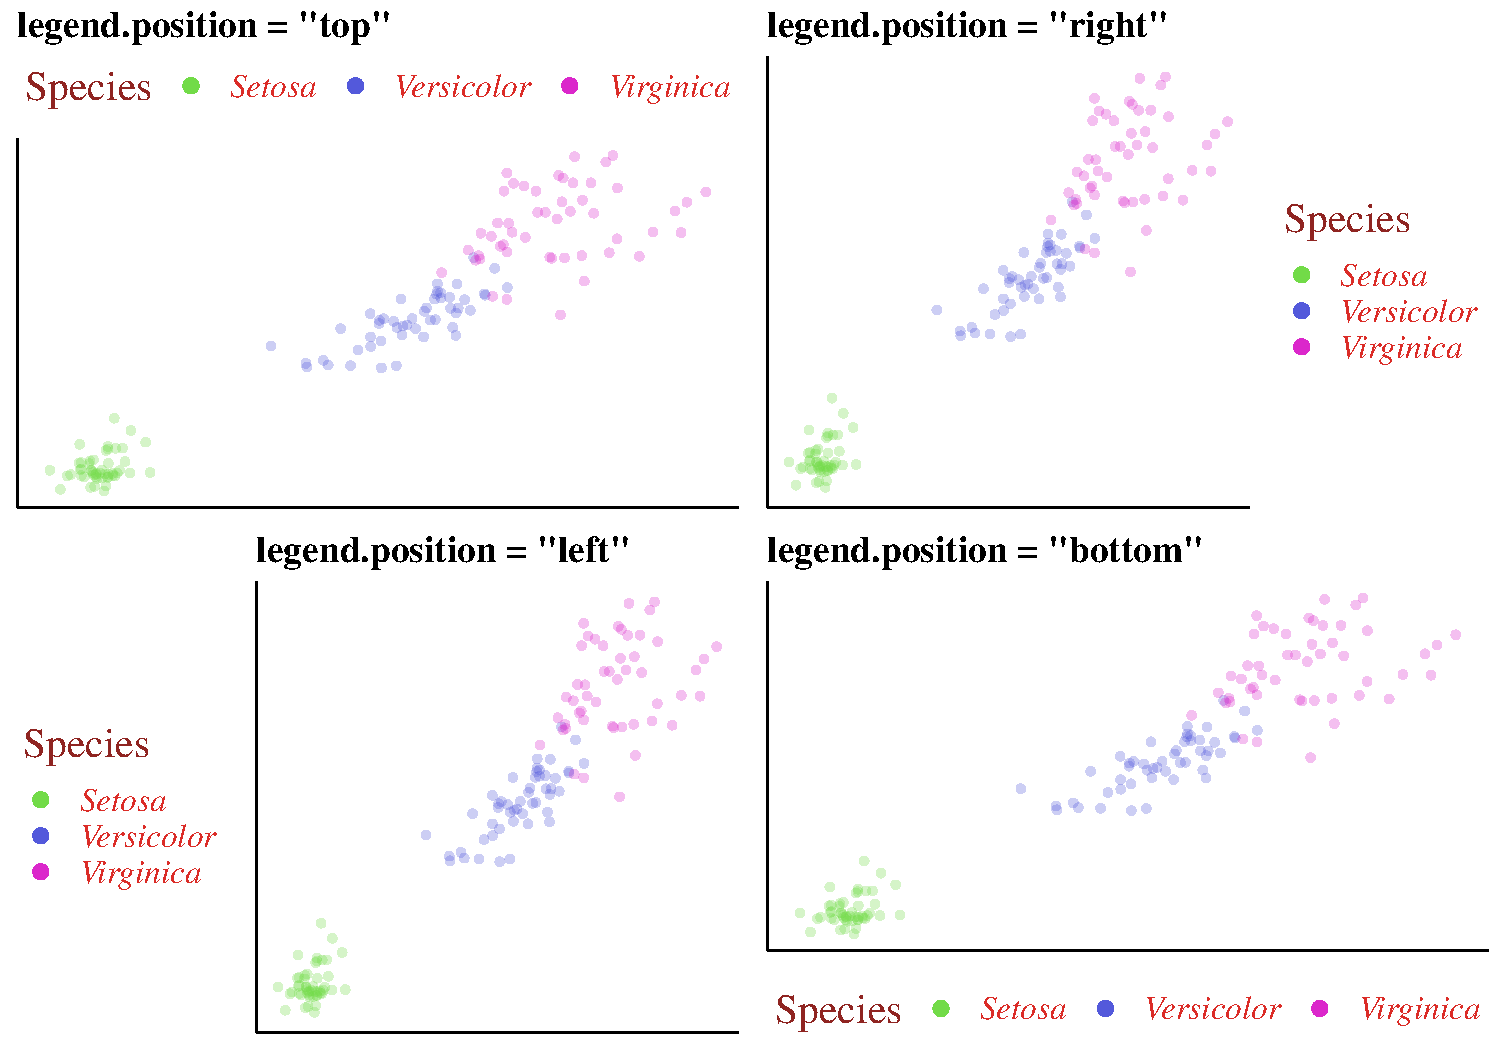
\includegraphics[width=0.99\linewidth]{PlotsLec3/LegPos}
\end{figure}
\end{frame}

\begin{frame}[fragile]{RCode to specify \texttt{\textcolor{red}{legend.position}}}
%\lstset{basicstyle=\Large\ttfamily}
\begin{lstlisting}
# Legend position at the top
theme(legend.position = "top")

# Legend position at the right
theme(legend.position = "right")

# Legend position at the left
theme(legend.position = "left")

# Legend position at the bottom
theme(legend.position = "bottom")

# Remove legend completely
theme(legend.position = "none")                  
\end{lstlisting}
\end{frame}

\setbeamercovered{transparent}
\begin{frame}\frametitle{Putting legend inside the plot}
\begin{itemize}
\item In most academic publication, the legends are required to be placed inside the plot.

\vspace{0.15in}

\item<2-> This is particularly useful when you have a lot of blank space in your plot.
\vspace{0.15in}

\item<3-> This can be achieved by passing a numeric vector with x and y coordinates to the \texttt{\textcolor{red}{legend.position}} parameter in the \texttt{\textcolor{red}{theme()}} layer.
\vspace{0.15in}

\item<4-> The x and y coordinates represent a relative location in the panel: 
\begin{enumerate}
\item \texttt{\textcolor{red}{c(0, 0)}} is bottom left;
\item \texttt{\textcolor{red}{c(0, 1)}} is top left;
\item \texttt{\textcolor{red}{c(1, 0)}} is bottom right;
\item \texttt{\textcolor{red}{c(1, 1)}} is top right.
\end{enumerate}
\end{itemize}
\end{frame}

\begin{frame}\frametitle{Example: legend inside the plot}
\begin{figure}
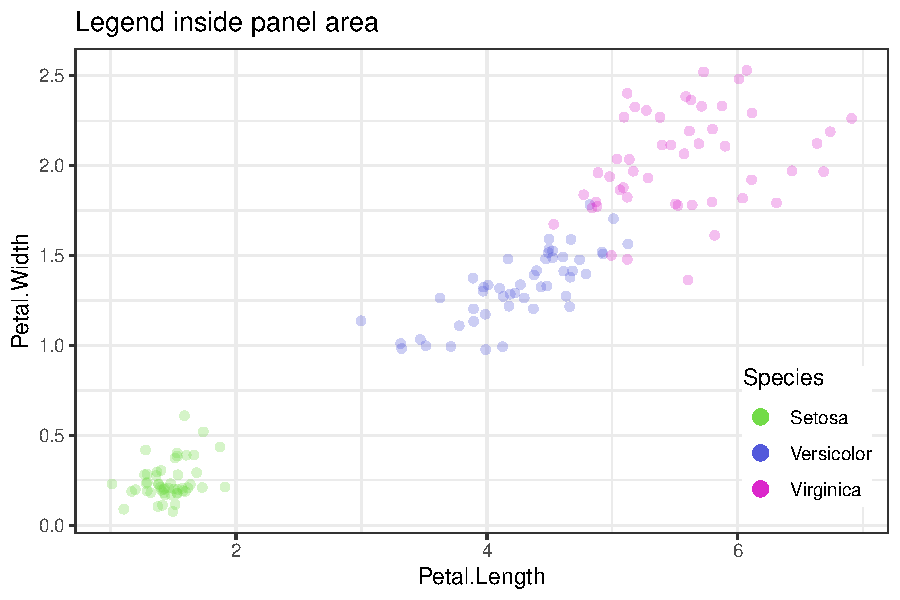
\includegraphics[width=0.99\linewidth]{PlotsLec3/LegPosInside}
\end{figure}
\end{frame}

\begin{frame}[fragile]{RCode: legend inside the plot}
%\lstset{basicstyle=\Large\ttfamily}
\begin{lstlisting}
####################################
# Specify legend position at the   #
# bottom right corner of the plot  #
####################################
theme(legend.position = c(0.9, 0.2),
####################################
# Remove the legend margin for     #
# an enhanced visualisation        #
####################################
legend.margin = margin(0,0,0,0,  "mm"))
\end{lstlisting}
\textcolor{red}{Note}: Specifying a suitable legend position this way would often require a lot of trial and error on your part.
\end{frame}


\section{Line elements}
\begin{frame}{\texttt{\textcolor{red}{line}} element hierarchy structure}
\begin{figure}
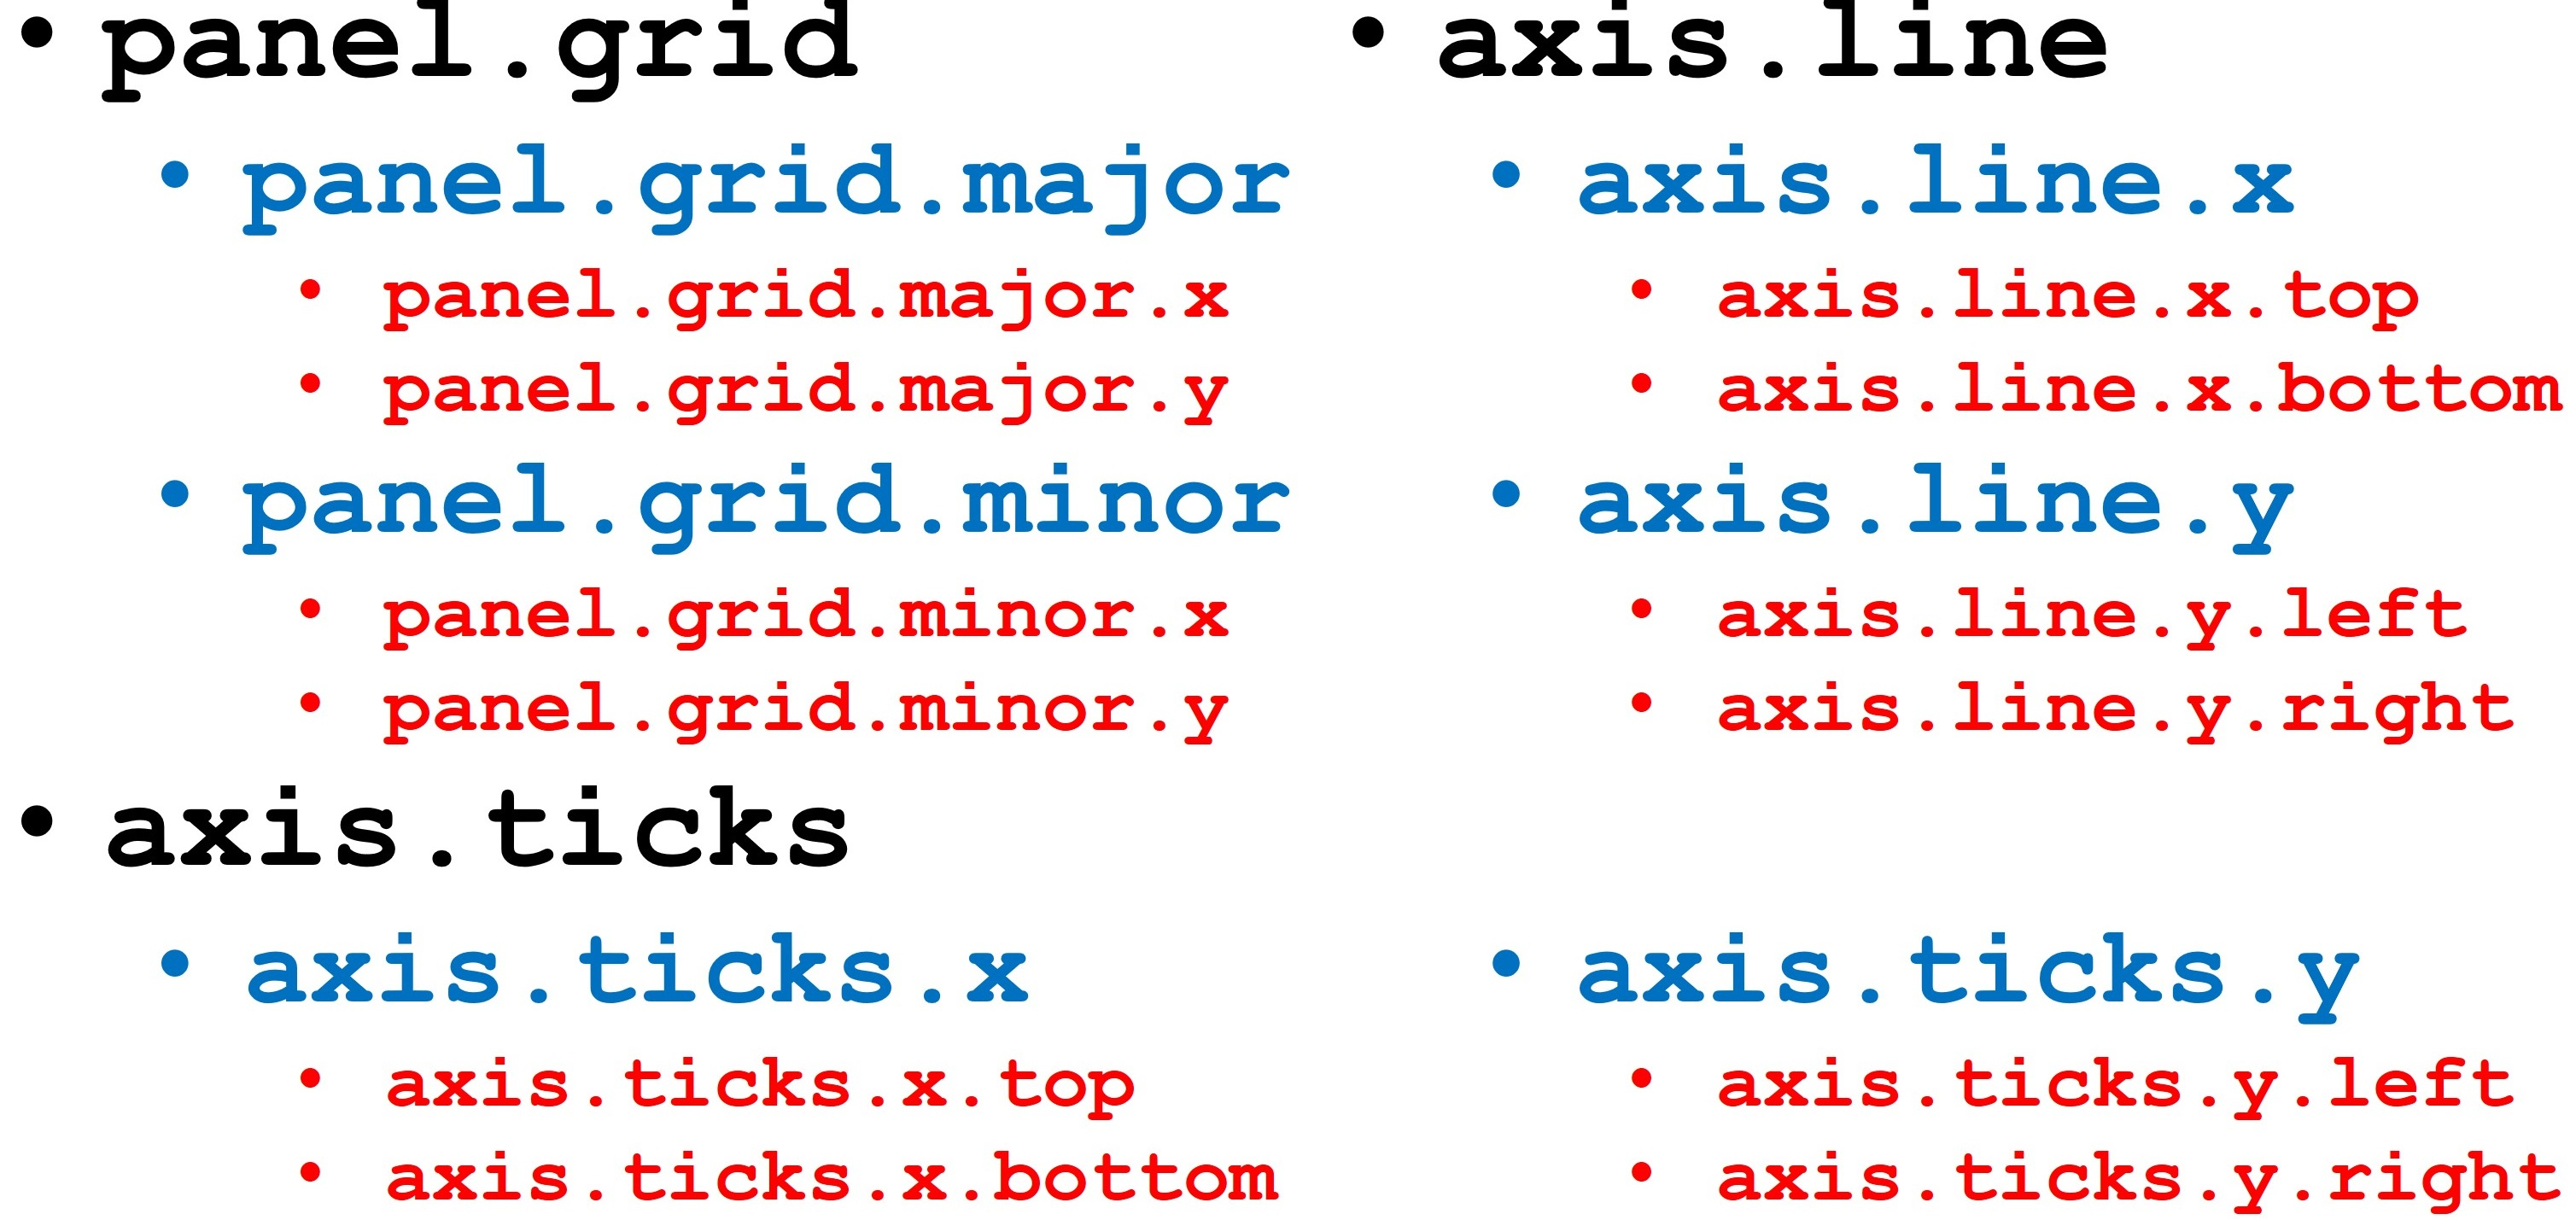
\includegraphics[width=0.99\linewidth]{PlotsLec3/LineThemeElements}
\caption{\small{Use \texttt{\textcolor{red}{element}$\_$\textcolor{red}{line()}} to modify all line elements}.}
\end{figure}
\end{frame}

\begin{frame}\frametitle{Modifying \texttt{\textcolor{red}{panel.grid}} lines}
We changed the color, size and linetype attributes of \texttt{\textcolor{red}{panel.grid}} lines.
\begin{figure}
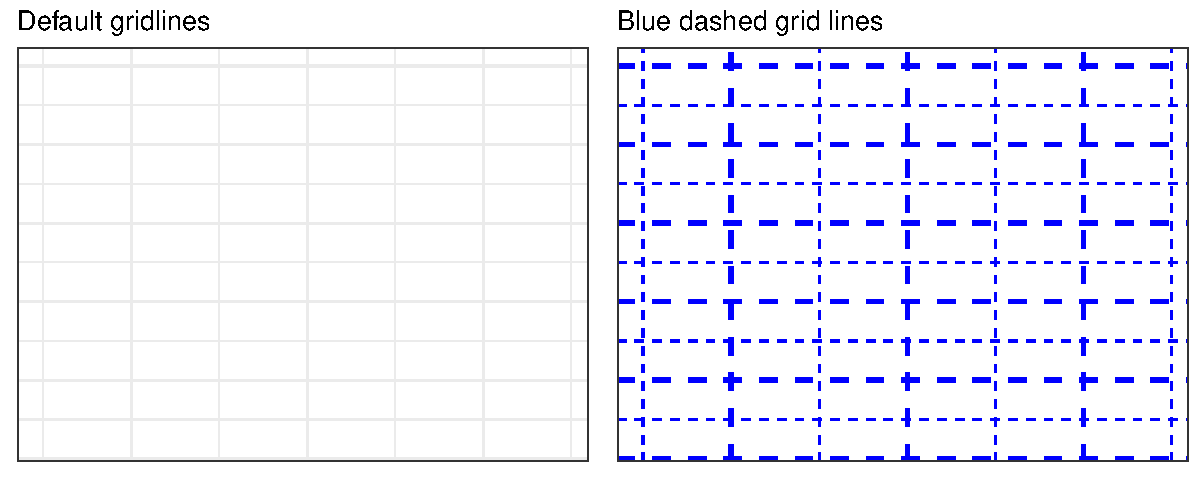
\includegraphics[width=0.99\linewidth]{PlotsLec3/GridLinePlt}
\caption{\small{Use \texttt{\textcolor{red}{panel.grid}} parameter inside \texttt{\textcolor{red}{theme()}} to modify both major and minor panel grid-lines}.}
\end{figure}
\end{frame}


\begin{frame}[fragile]{RCode: modify \texttt{\textcolor{red}{panel.grid}} lines}
%\lstset{basicstyle=\Large\ttfamily}
\begin{lstlisting}
#####################################
# Specify panel grid line attributes#
#####################################
mygrid <- element_line(color = "blue",
                       size = 1,
                    linetype = "dashed")
#####################################
# Use panel.grid parameter inside   #
# theme() layer to modify grid lines#
#####################################
theme(panel.grid = mygrid)
\end{lstlisting}
\end{frame}

\setbeamercovered{transparent}
\begin{frame}\frametitle{Modify height of \texttt{\textcolor{red}{axis.ticks}}}
\begin{itemize}
\item Because axis ticks are treated as line elements, these can be modified using \texttt{\textcolor{red}{element}$\_$\textcolor{red}{line()}} like any other line elements.
\vspace{0.2in}

\item<2-> However, to modify the height of the axis ticks, we need to use the \texttt{\textcolor{red}{axis.ticks.length}} parameter
of the \texttt{\textcolor{red}{theme()}} layer.
\vspace{0.2in}

\item<3-> The \texttt{\textcolor{red}{axis.ticks.length}} parameter accepts an object of the class \texttt{\textcolor{red}{unit()}}.
\vspace{0.2in}

\item<4-> The first argument of  \texttt{\textcolor{red}{unit()}} is a length value, and the second argument is a length unit. For example, to specify 1 cm, we shall use \texttt{\textcolor{red}{unit(1, "cm")}}.
\end{itemize}

\end{frame}

\begin{frame}\frametitle{Modifying \texttt{\textcolor{red}{axis.ticks.length}}}
\begin{figure}
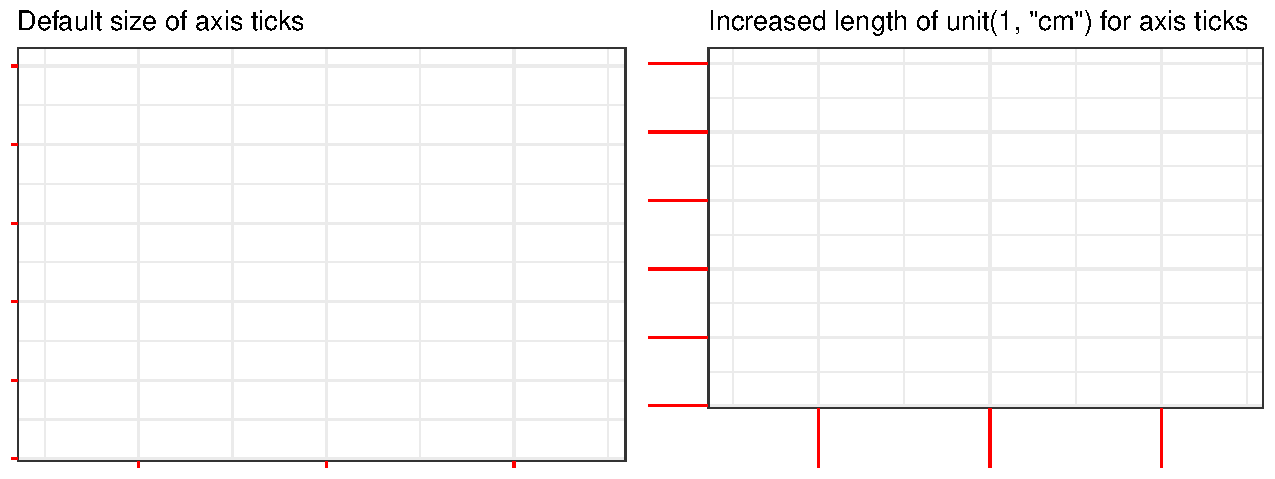
\includegraphics[width=0.99\linewidth]{PlotsLec3/AxisTicksPlt}
\caption{\small{\texttt{\textcolor{red}{axis.ticks.length = unit(1, "cm")}} is used inside the \texttt{\textcolor{red}{theme()}} layer to modify the length of axis ticks}.}
\end{figure}
\end{frame}


\section{Rectangular elements}
\begin{frame}{\texttt{\textcolor{red}{rect}} element hierarchy structure}
\begin{figure}
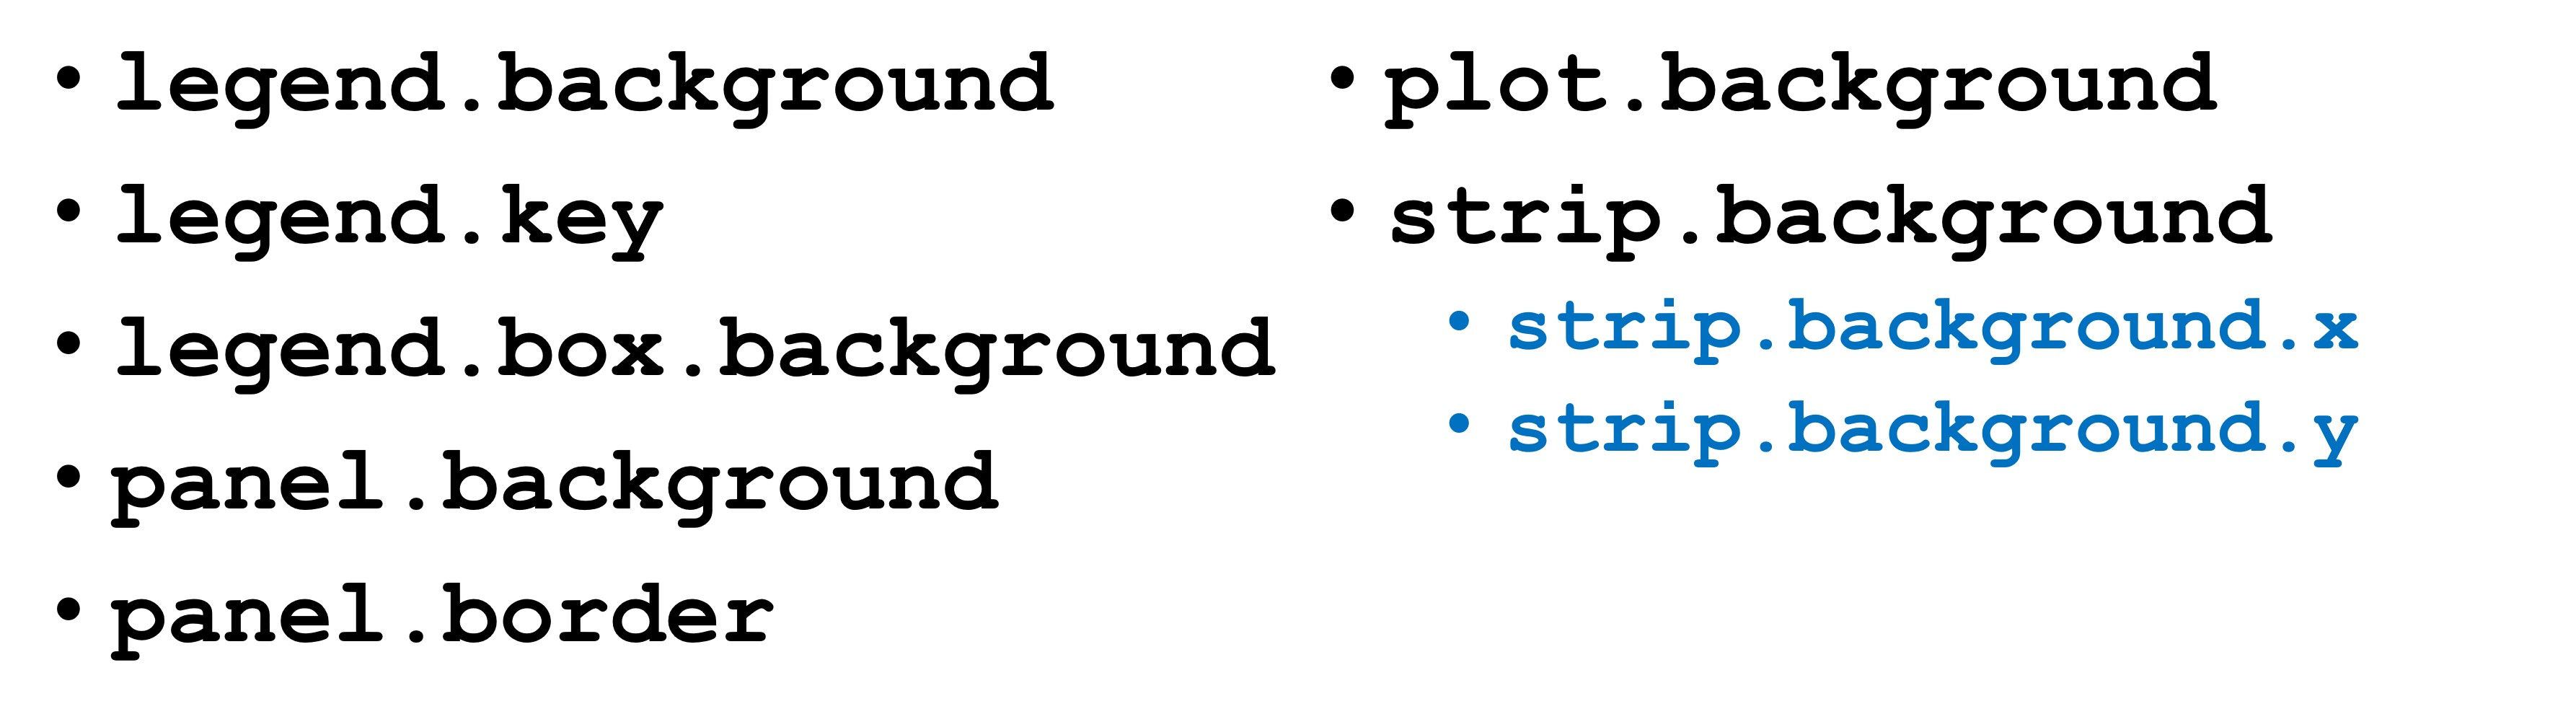
\includegraphics[width=0.99\linewidth]{PlotsLec3/RectThemeElements}
\caption{\small{Use \texttt{\textcolor{red}{element}$\_$\textcolor{red}{rect()}} to modify all rectangular elements}.}
\end{figure}
\end{frame}

\section{Custom theme creation}

\begin{frame}{Create customised theme -- Curtin theme}
We have created a customised theme inspired by the colors prominent in the Curtin University logo.
\begin{figure}
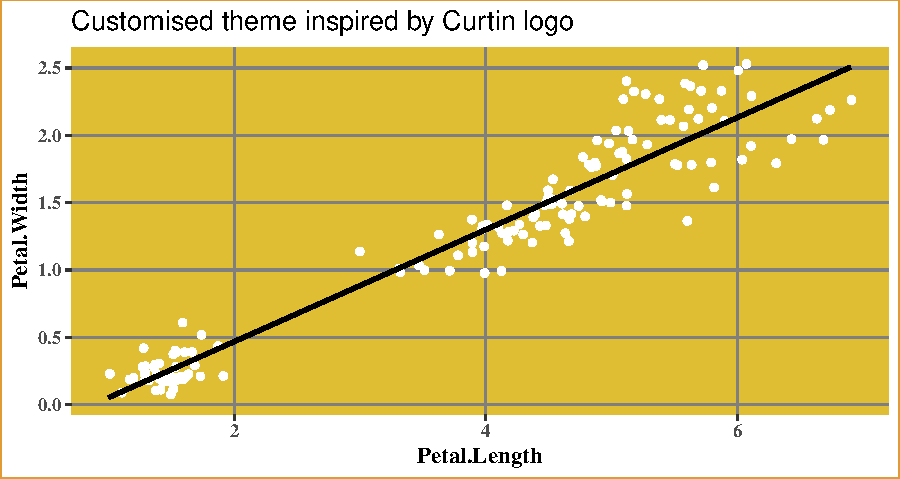
\includegraphics[width=0.99\linewidth]{PlotsLec3/CurtinThemePlt}
\caption{\small{Relationship between iris Petal.Width and Petal.Length, fitted using the linear regression model.}}
\end{figure}
\end{frame}

\begin{frame}[fragile]{RCode: create Curtin theme}
%\lstset{basicstyle=\Large\ttfamily}
\begin{lstlisting}
# Create custom theme
curtin_theme <-
theme(plot.background = 
      	element_rect(color = "#E09B34"),
     panel.background = 
      	element_rect(fill = "#E0BE34"),
     panel.grid.major = 
      	element_line(color = "gray50"),
     panel.grid.minor = element_blank(),
     axis.text = 
        element_text(face = "bold",
                     family = "serif"),
     axis.title = 
        element_text(face = "bold",
                     family = "serif"))
\end{lstlisting}
\end{frame}

\begin{frame}[fragile]{RCode: use Curtin theme to plot}
%\lstset{basicstyle=\Large\ttfamily}
\begin{lstlisting}
# Plot Petal.Width vs Petal.Length
ggplot(iris, 
       aes(x = Petal.Length,
           y = Petal.Width)) +
# Add jittered points
geom_point(position = 
            position_jitter(seed = 123), 
            color = "white",
            size = 1.3) +
# Add the line of best fit
geom_smooth(method = "lm", 
            se = FALSE, 
            color = "black") +
# Add Curtin theme object
curtin_theme
\end{lstlisting}
\end{frame}

\section{Ggplot2 in-built themes and others}

\begin{frame}{Use ggplot2 in-built themes}
\begin{figure}
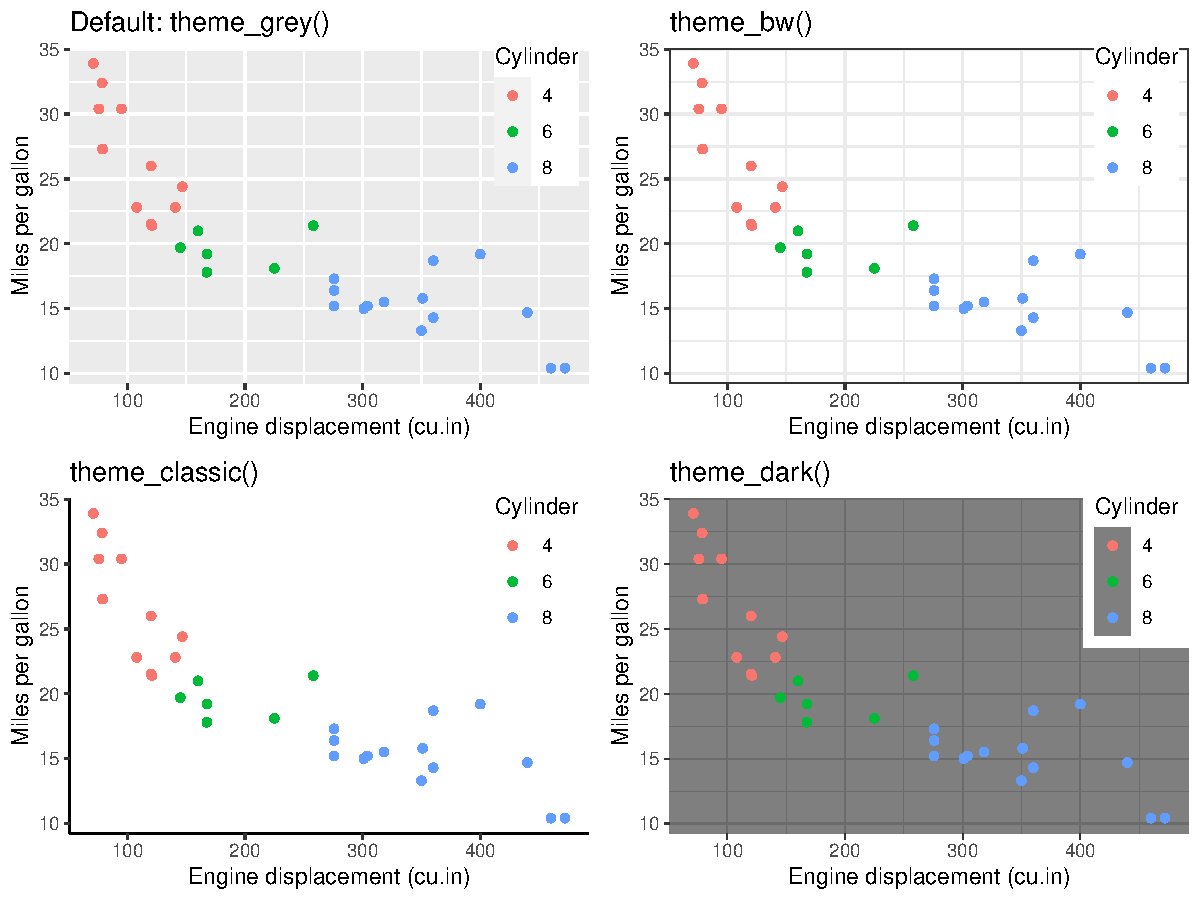
\includegraphics[width=0.99\linewidth]{PlotsLec3/InBuiltTheme}
\end{figure}
\end{frame}



\begin{frame}{Use \texttt{\textcolor{red}{ggthemes}} package for more themes}
\begin{figure}
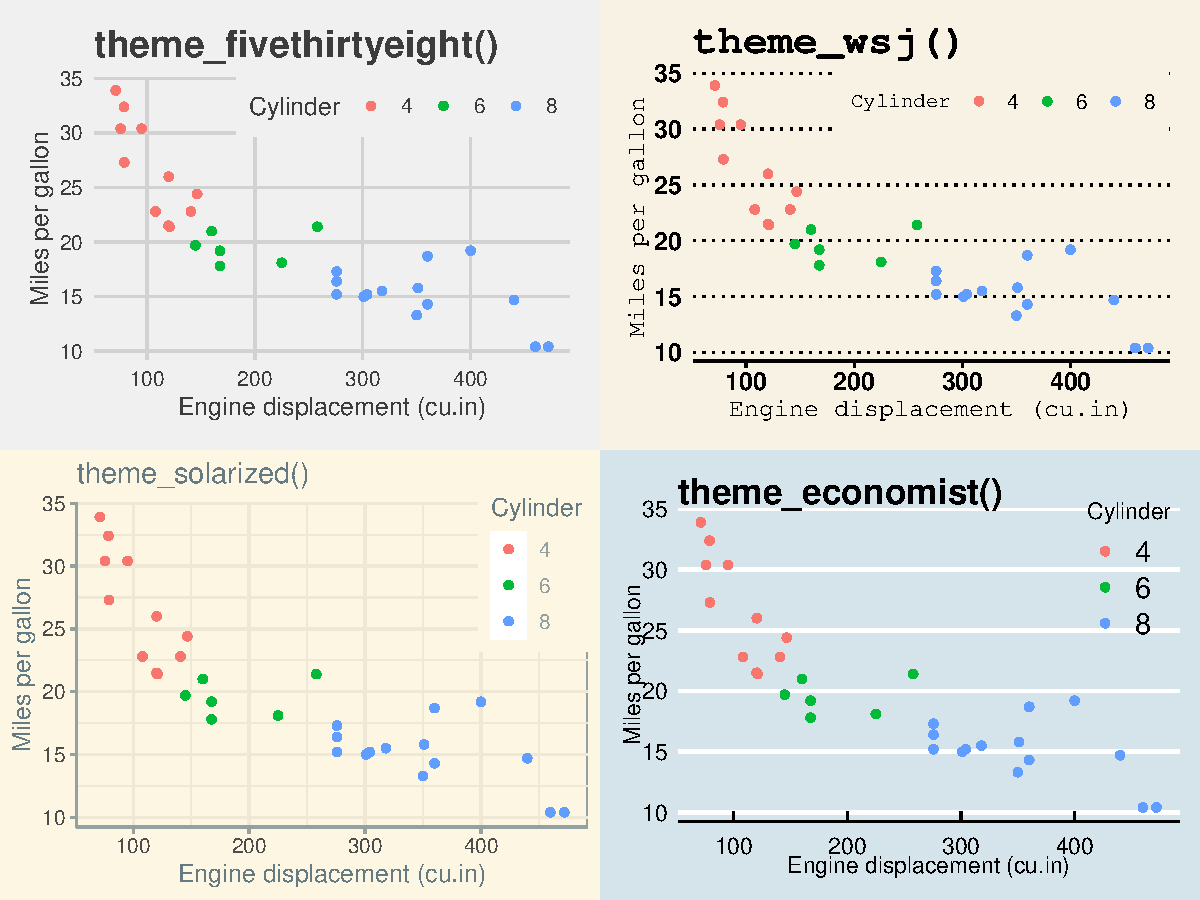
\includegraphics[width=0.99\linewidth]{PlotsLec3/InBuiltTheme2}
\end{figure}
\end{frame}

\setbeamercovered{transparent}
\begin{frame}{Important \texttt{\textcolor{red}{scale$\_\star \_\star()$}} class of functions}
\begin{itemize}
\item We have seen that \texttt{\textcolor{red}{aes()}} is used to \textcolor{blue}{map variables to visual aesthetics}. The \texttt{\textcolor{red}{scale}} functions are used to modify or enhance this mapping.
\vspace{0.3in}
\item<2-> For every aesthetic, we have corresponding \texttt{\textcolor{red}{scale}} functions. For example, for the \texttt{\textcolor{red}{x}} and \texttt{\textcolor{red}{y}} aesthetics, the corresponding scales functions are of the forms \texttt{\textcolor{red}{scale$\_$x$\_\star()$}} and \texttt{\textcolor{red}{scale$\_$y$\_\star()$}}, respectively.
\vspace{0.3in}
\item<3-> The last \textcolor{red}{$\star$} corresponds to the type of variable that is mapped to the visual aesthetic. For example, if a continuous variable is mapped to the \texttt{\textcolor{red}{x}} axis, then the corresponding scale function is \texttt{\textcolor{red}{scale$\_$x$\_$continuous()}}. 
\end{itemize}
\end{frame}

\section{Important scale functions}
%\setbeamercovered{transparent}
\begin{frame}{Useful arguments of \texttt{\textcolor{red}{scale$\_$x$\_$continuous()}}}
\begin{itemize}
\item \texttt{\textcolor{red}{trans}}: name of the transformation, e.g., \texttt{\textcolor{red}{"log10"}}, \texttt{\textcolor{red}{"sqrt"}}, and \texttt{\textcolor{red}{"log"}}.
\vspace{0.3in}

\item \texttt{\textcolor{red}{breaks}}: a numeric vector of positions for axis labels to appear.
\vspace{0.3in}

\item \texttt{\textcolor{red}{labels}}: a character vector giving labels (must be same length as \texttt{\textcolor{red}{breaks}}).

\vspace{0.3in}
\item \texttt{\textcolor{red}{position}}: the position of the axis, e.g., \texttt{\textcolor{red}{"top"}} or \texttt{\textcolor{red}{"bottom"}} for the \texttt{\textcolor{red}{x}}-axis.
\end{itemize}
\end{frame}

\begin{frame}{Example: Diamond price vs $\log10$(carat)}
We used \texttt{\textcolor{red}{scale$\_$x$\_$continuous()}} to transform the x-axis into $\log10$ scale, and used the \texttt{\textcolor{red}{scale$\_$y$\_$continuous()}} to change the y-axis labels.
\begin{figure}
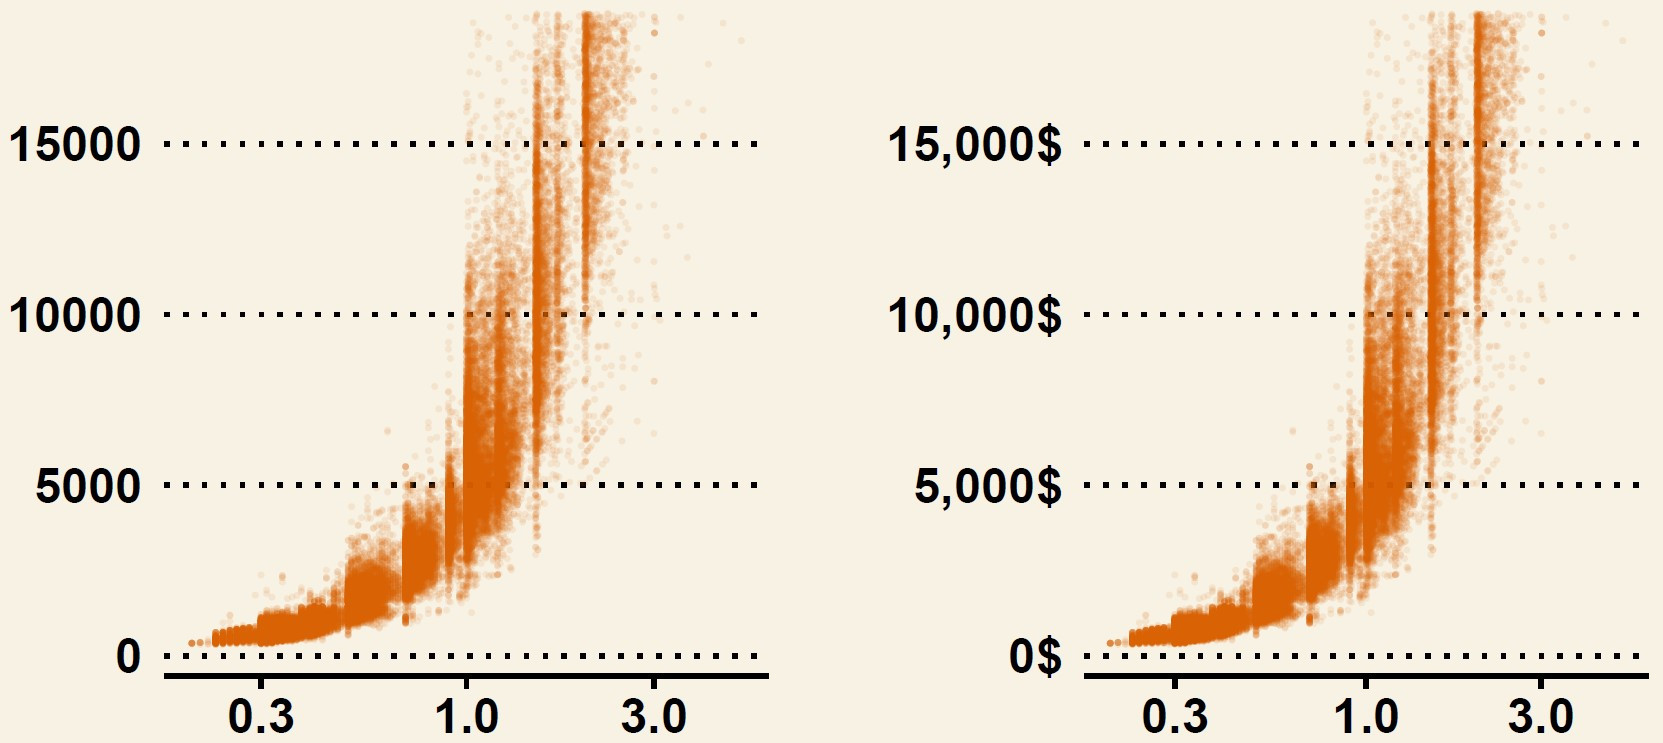
\includegraphics[width=0.99\linewidth]{PlotsLec3/DiamondExample}
\caption{\small{\textit{Left}: Default y-axis labels; \textit{Right}: Dollar sign and comma are added to the price for visual enhancement}}.
\end{figure}
\end{frame}

\begin{frame}[fragile]{RCode: \texttt{\textcolor{red}{scale$\_$y$\_$continuous()}} example}
%\lstset{basicstyle=\Large\ttfamily}
\begin{lstlisting}
# Plot diamond price vs log10(carat)
ggplot(diamonds, aes(carat, price)) +
geom_point(size = 0.1, 
           alpha=0.10, 
           color = "#D55E00") +
# Change x-axis to log-scale
scale_x_continuous(
   "log10(carat)",
   trans = "log10") +
# Change y-axis labels
scale_y_continuous(
   breaks = c(0, 5000, 10000, 15000),
   labels = c("0$", "5,000$", 
              "10,000$", "15,000$")) +
theme_wsj()
\end{lstlisting}
\end{frame}

\setbeamercovered{transparent}
\begin{frame}{\texttt{\textcolor{red}{scale$\_$color$\_\star$()}} functions}
\begin{itemize}
\item \texttt{\textcolor{red}{scale$\_$color$\_$brewer()}} and \texttt{\textcolor{red}{scale$\_$color$\_$manual()}} are two useful functions that allow us to change the default color produced by mapping to the color aesthetics. 

\item<2-> The \texttt{\textcolor{red}{scale$\_$color$\_$brewer()}} provides sequential, diverging and qualitative color schemes from the R-package \texttt{\textcolor{red}{RColorBrewer}}.

\item<3-> Modify the \texttt{\textcolor{red}{type}} and \texttt{\textcolor{red}{palette}} argument inside \texttt{\textcolor{red}{scale$\_$color$\_$brewer()}}:
\begin{itemize}
\item \texttt{\textcolor{red}{type}} -- one of \textcolor{blue}{``seq"} (sequential), \textcolor{blue}{``div"} (divergent), and \textcolor{blue}{``qual"} (qualitative).
\item \texttt{\textcolor{red}{palette}} -- If a string, will use the named palette. If a number, will index into the list of palettes of appropriate \texttt{\textcolor{red}{type}}.
\begin{itemize}
\item \textcolor{blue}{Diverging}: BrBg, PiYG, RdYlBu, RdYlGr, Spectral.
\item \textcolor{blue}{Qualitative}: Accent, Set1, Set2, Pastel1.
\item \textcolor{blue}{Sequential}: Blues, YlOrRd, YlGnBu, Purples.
\end{itemize}
\end{itemize}
\end{itemize}
\end{frame}


\begin{frame}{Example: \texttt{\textcolor{red}{scale$\_$color$\_$brewer()}}}
\begin{figure}
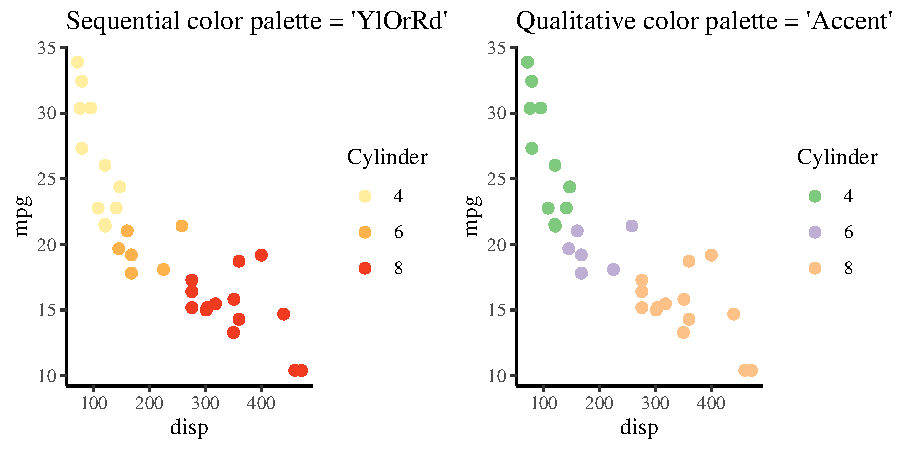
\includegraphics[width=0.99\linewidth]{PlotsLec3/ColorBrewer}
\caption{\small{\textit{Left}: Sequential color palette used; \textit{Right}: Qualitative color palette used}}.
\end{figure}
\end{frame}

\begin{frame}[fragile]{RCode: \texttt{\textcolor{red}{scale$\_$color$\_$brewer()}} example}
%\lstset{basicstyle=\Large\ttfamily}
\begin{lstlisting}
baseplt <- ggplot(mtcars,aes(disp, mpg, 
              color = factor(cyl))) +
           geom_point()
# Use a sequential palette
baseplt +
scale_color_brewer("Cylinder", 
                    type = "seq", 
                    palette = "YlOrRd")
# Use a qualitative palette
baseplt +
scale_color_brewer("Cylinder", 
                   type = "qual", 
                   palette = "Accent")
\end{lstlisting}
\end{frame}

\setbeamercovered{transparent}
\begin{frame}{\texttt{\textcolor{red}{scale$\_$color$\_$manual()}} function}
\begin{itemize}
\item \texttt{\textcolor{red}{scale$\_$color$\_$manual()}} provides the most flexibility, as it allows you to create own discrete color scale.
\vspace{0.25in}
\item<2-> The two most important parameters are \texttt{\textcolor{red}{values}} and \texttt{\textcolor{red}{breaks}}:
\begin{itemize}
\item \texttt{\textcolor{red}{values}}: for a categorical variable, provide a vector specifying colors for each category; for a continuous variable, provide a vector specifying colors for number of categories created by the number of \texttt{\textcolor{red}{breaks}};
\item \texttt{\textcolor{red}{breaks}}: levels for which a color band is specified.
\end{itemize}
\vspace{0.25in}

\item<3-> Similarly, for \texttt{\textcolor{red}{fill}} aesthetics, we have \texttt{\textcolor{red}{scale$\_$fill$\_$brewer()}} and 
\texttt{\textcolor{red}{scale$\_$fill$\_$manual()}} functions.
\end{itemize}
\end{frame}

\begin{frame}{Example: \texttt{\textcolor{red}{scale$\_$color$\_$manual()}}}
\begin{figure}
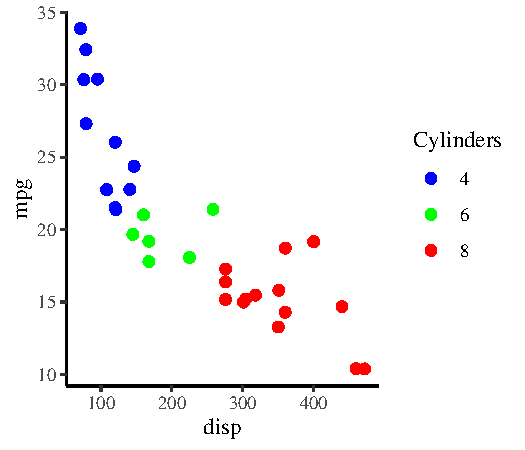
\includegraphics[width=0.80\linewidth]{PlotsLec3/ColorManual}
\caption{\small{User-specified discrete color scale for three cylinder numbers in the mtcars dataset}.}.
\end{figure}
\end{frame}

\begin{frame}[fragile]{RCode: \texttt{\textcolor{red}{scale$\_$color$\_$manual()}} example}
%\lstset{basicstyle=\Large\ttfamily}
\begin{lstlisting}
baseplt <- ggplot(mtcars,aes(disp, mpg, 
           color = factor(cyl))) +
           geom_point()

# Define a named vector with your favourite colors
col_vec <- c("4" = "blue",
             "6" = "green", 
             "8" = "red")

# Use your favourite colors
baseplt +
 scale_color_manual("Cylinders",
                    values = col_vec)
                    
\end{lstlisting}
\end{frame}

\section{Summary}
\begin{frame}\frametitle{Summary}
\begin{itemize}
\item Theme elements are all non-data ink in the plot.
\item Use \texttt{\textcolor{red}{element}$\_$\textcolor{red}{text()}}, \texttt{\textcolor{red}{element}$\_$\textcolor{red}{line()}}, and \texttt{\textcolor{red}{element}$\_$\textcolor{red}{rect()}} to modify three main theme elements.

\item You can specify plot title, tag, caption, legend title, axis title in the \textcolor{red}{\texttt{labs()}} function.

\item Use \texttt{\textcolor{red}{override.aes}} parameter of \texttt{\textcolor{red}{guide}$\_$\textcolor{red}{legend()}} to modify legend guides.

\item You can build custom themes or use many in-built themes from different R-packages. 

\item Use \textcolor{red}{\texttt{scale}} functions to modify the default aesthetic mappings.

\item Use \texttt{\textcolor{red}{scale$\_$color$\_$manual()}} to select customised colors for the plot.
\end{itemize}
\end{frame}


\end{document} 